\documentclass[12pt]{book}

\usepackage[utf8]{inputenc}
\usepackage[T1]{fontenc}
\usepackage{geometry}
\usepackage{graphicx}
\usepackage[spanish, es-tabla]{babel}
\usepackage{amsthm}
\usepackage{amsmath}
\usepackage{trfsigns}
\usepackage{amssymb}


%Para listado de programas
\usepackage{listings}
\usepackage{color}

\definecolor{mygreen}{rgb}{0.95,0.9,0}
\definecolor{mygray}{rgb}{0.7,0.7,0.7}
\definecolor{mymauve}{rgb}{0.58,0,0.82}

\lstset{ %
	 backgroundcolor=\color{mygreen},   % choose the background color; you must add \usepackage{color} or \usepackage{xcolor}
	 basicstyle=\footnotesize\ttfamily,        % the size of the fonts that are used for the code
	 breaklines=true,            % Zeilen werden Umgebrochen
	 keywordstyle=\color{red},
	 commentstyle=\itshape\color{mygreen},    % comment style
	 numbers=left,                    % where to put the line-numbers; possible values are (none, left, right)
	 numbersep=5pt                   % how far the line-numbers are from the code
}



\newtheorem{thm}{Teorema}[section]
\theoremstyle{definition}
\newtheorem{dfn}{Definición}[section]
\theoremstyle{remark}
\newtheorem{note}{Nota}[section]
\theoremstyle{plain}
\newtheorem{lem}[thm]{Lema}

\geometry{letterpaper}



%un estilo propio
\usepackage{fancyhdr}
\setlength{\headheight}{15pt}

\pagestyle{fancy}
\renewcommand{\chaptermark}[1]{ \markboth{\chaptername\ \thechapter: #1}{} }
\renewcommand{\sectionmark}[1]{ \markright{ Sección \thesection. #1}{} }

\fancyhf{}
\fancyhead[LE,RO]{\thepage}
\fancyhead[RE]{\textit{ \nouppercase{\leftmark}} }
\fancyhead[LO]{\textit{ \nouppercase{\rightmark}} }
\fancyfoot[CE]{\textit{\textcopyright 2022\\
		Naktan} }
\fancyfoot[CO]{\textit{Departamento de I+D, SMARTEST \\
		Elaboró: Dr. Casimiro Gómez González} }	            
\fancypagestyle{plain}{ %
	\fancyhf{} % remove everything
	\renewcommand{\headrulewidth}{0pt} % remove lines as well
	\renewcommand{\footrulewidth}{0pt}
}

\title{Aplicaciones con RUST}
\author{Dr. Casimiro Gómez González\\
	Departamento de I+D, SMARTEST\\
               correo: casimiro.gomez@smartest.mx\\
               Tel: 222 707 4118}
\date{Primavera 2022}

\begin{document}
\frontmatter
\maketitle


\chapter{Prólogo}

El presente proyecto presenta las bases del desarrollo de un \textbf{API} basado en RUST. Los conceptos básicos del API han sido desarrollado a lo largo del presente documento desde sus bases hasta la primera aplicación de envío de correos. 
´
\begin{flushright}

El autor\\
Casimiro Gómez González\\
Departamento de I+D, \textbf{SMARTEST}
\end{flushright}

\tableofcontents

\mainmatter


\chapter{Diseño de la estructura APP}
En el presente capítulo se realizarán las configuraciones iniciales de un proyecto en flutter.

\section{Creación del proyecto}

Vamos a crear el app de fluter para comercio electrónico de smartest, el proyecto se llama \textbf{vecnu} \footnote{Lo cual en el idioma lojban significa vender}. Para ello en una terminal, con una máquina que previamente tiene flutter instalado, ejecutamos:


\begin{lstlisting}[language=bash]
$ mkdir Vecnu 
$ cd Vecnu
$ flutter create vecnu
\end{lstlisting}

Para editar el proyecto se utiliza \emph{\textbf{visual studio code}}, por lo cual ejecutamos:

\begin{lstlisting}[language=bash]
$ cd vecnu
$ code .
\end{lstlisting}

Anteriormente se instalá a \emph{\textbf{visual studio code}} la extensión \textbf{flutter dev tools}. Apretamos las teclas \textbf{ctr->shift-> p} y escribimos \textbf{Flutter: Launch emulator} y nos permite seleccionar los emuladores que instalamos desde \textbf{android studio}, en nuestro caso el de pixel, quedando como se muestra en la figura \ref{cap1:001}.

\begin{figure}[htb]
\centering
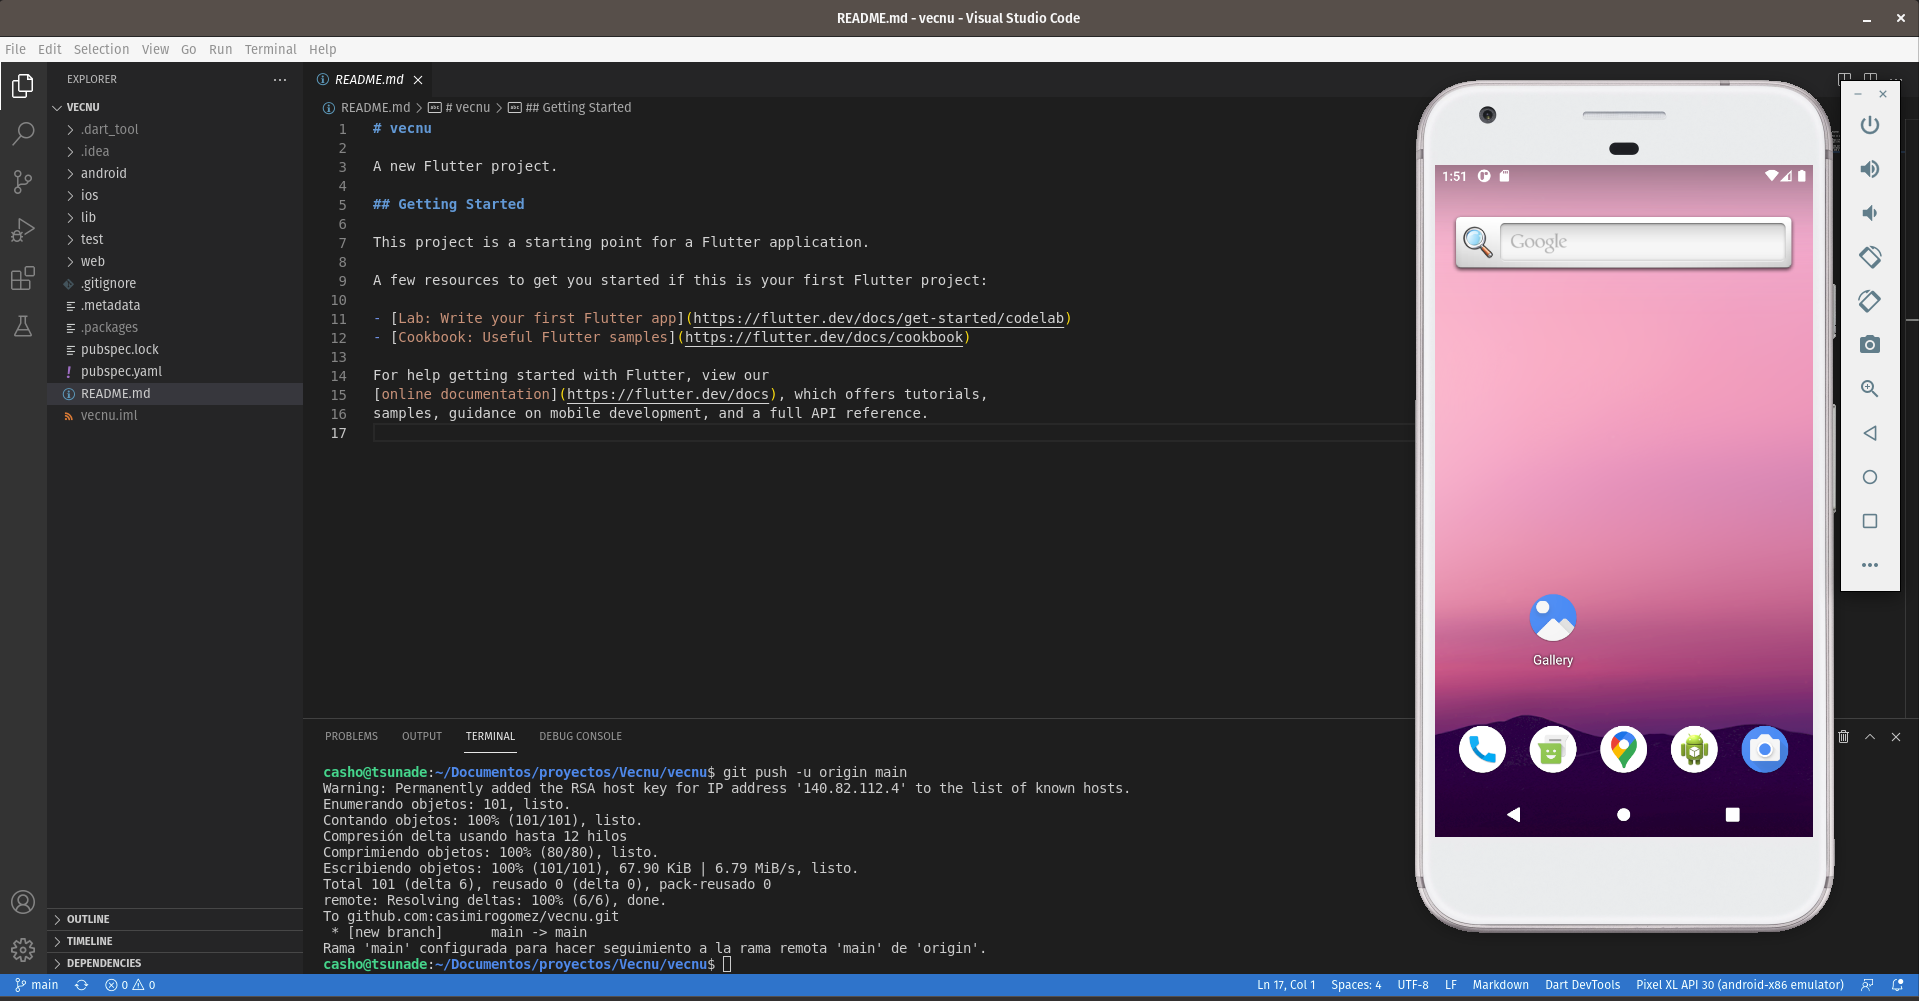
\includegraphics[width=0.7\textwidth]{capitulo1/emulador_1.png}
\caption{Programa creado y editando en \emph{\textbf{visual studio code}} y mostrando el emulador}
\label{cap1:001}
\end{figure} 

Para empezar a trabajar con el proyecto activamos la opción de debug, para ellos nuevamente apretamos las teclas \textbf{ctr->shift-> p} y escribimos \textbf{Debug: Start Debugging}, lo cual nos permite ejecutar nuestro proyecto en el emulador previamente abierto.

\begin{figure}[htb]
\centering
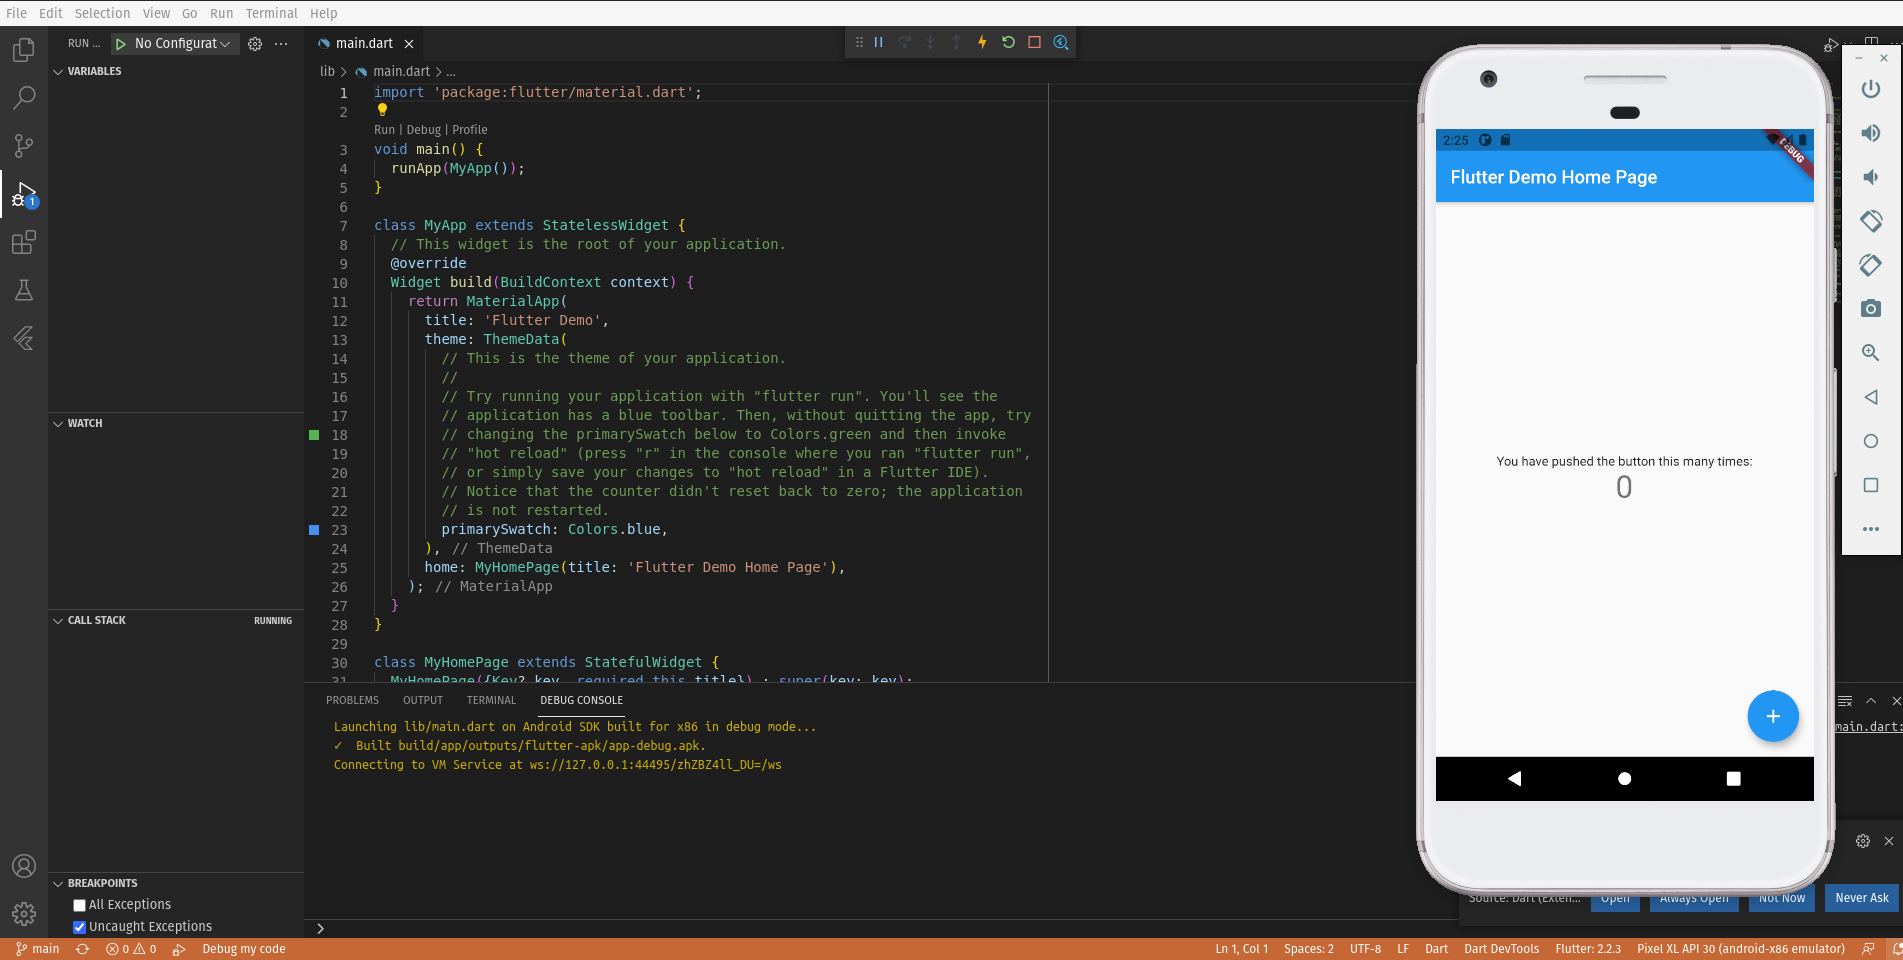
\includegraphics[width=0.6\textwidth]{capitulo1/emulador_corriendo.png}
\caption{Programa ejecutandose en el emulador}
\label{cap1:002}
\end{figure} 

Para que el debugger se ejecute correctamente necesitamos tener instalado Java en nuestra distribución de linux.

\section{Creando los temas para nuestro proyecto}

Para probar como se verán los colores en nuestra aplicación se usa la herramienta \textbf{Material Design Color Tool} la cual se encuentra en la dirección \emph{https://material.io /resources /color/ } en donde se seleccionan los colores primarios y secundarios para nuestra aplicación. En el caso de SMARTEST en la figura \ref{cap1:003} se muestra el código de colores.

\begin{figure}[htb]
\centering
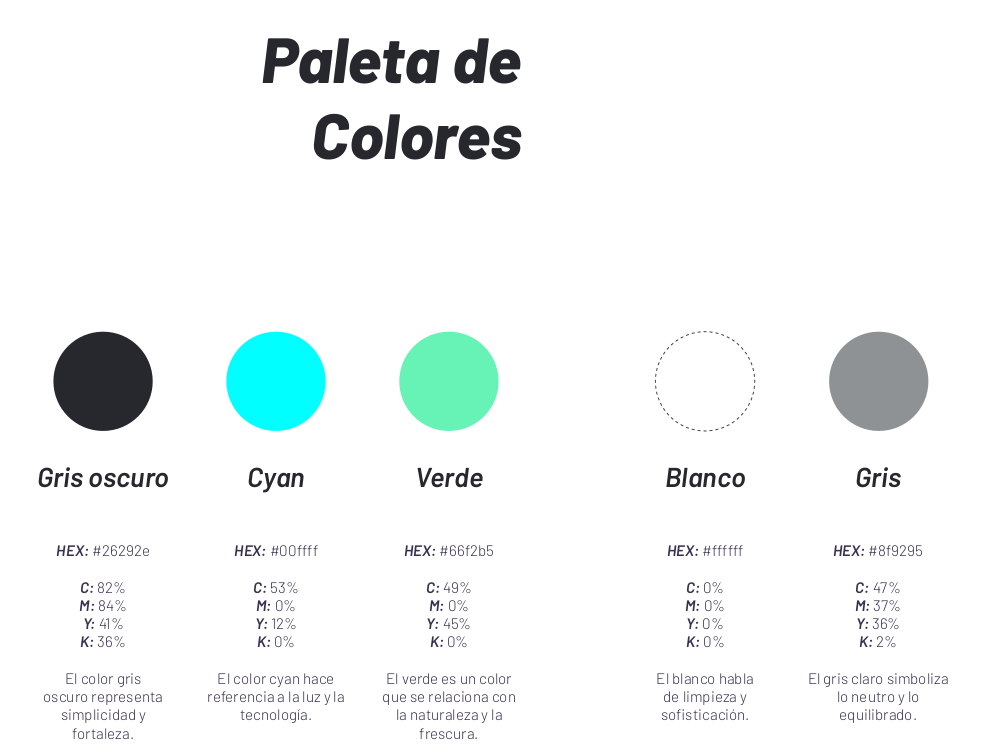
\includegraphics[width=0.6\textwidth]{capitulo1/paleta.png}
\caption{Paleta de colores}
\label{cap1:003}
\end{figure} 

De la figura \ref{cap1:003} se toman dos colores el cyan y el gris, y se forman los colores de la aplicación. Una vez decididos los colores de la aplicación y probados en la página. Se procede a programar el app.

\begin{figure}[htb]
\centering
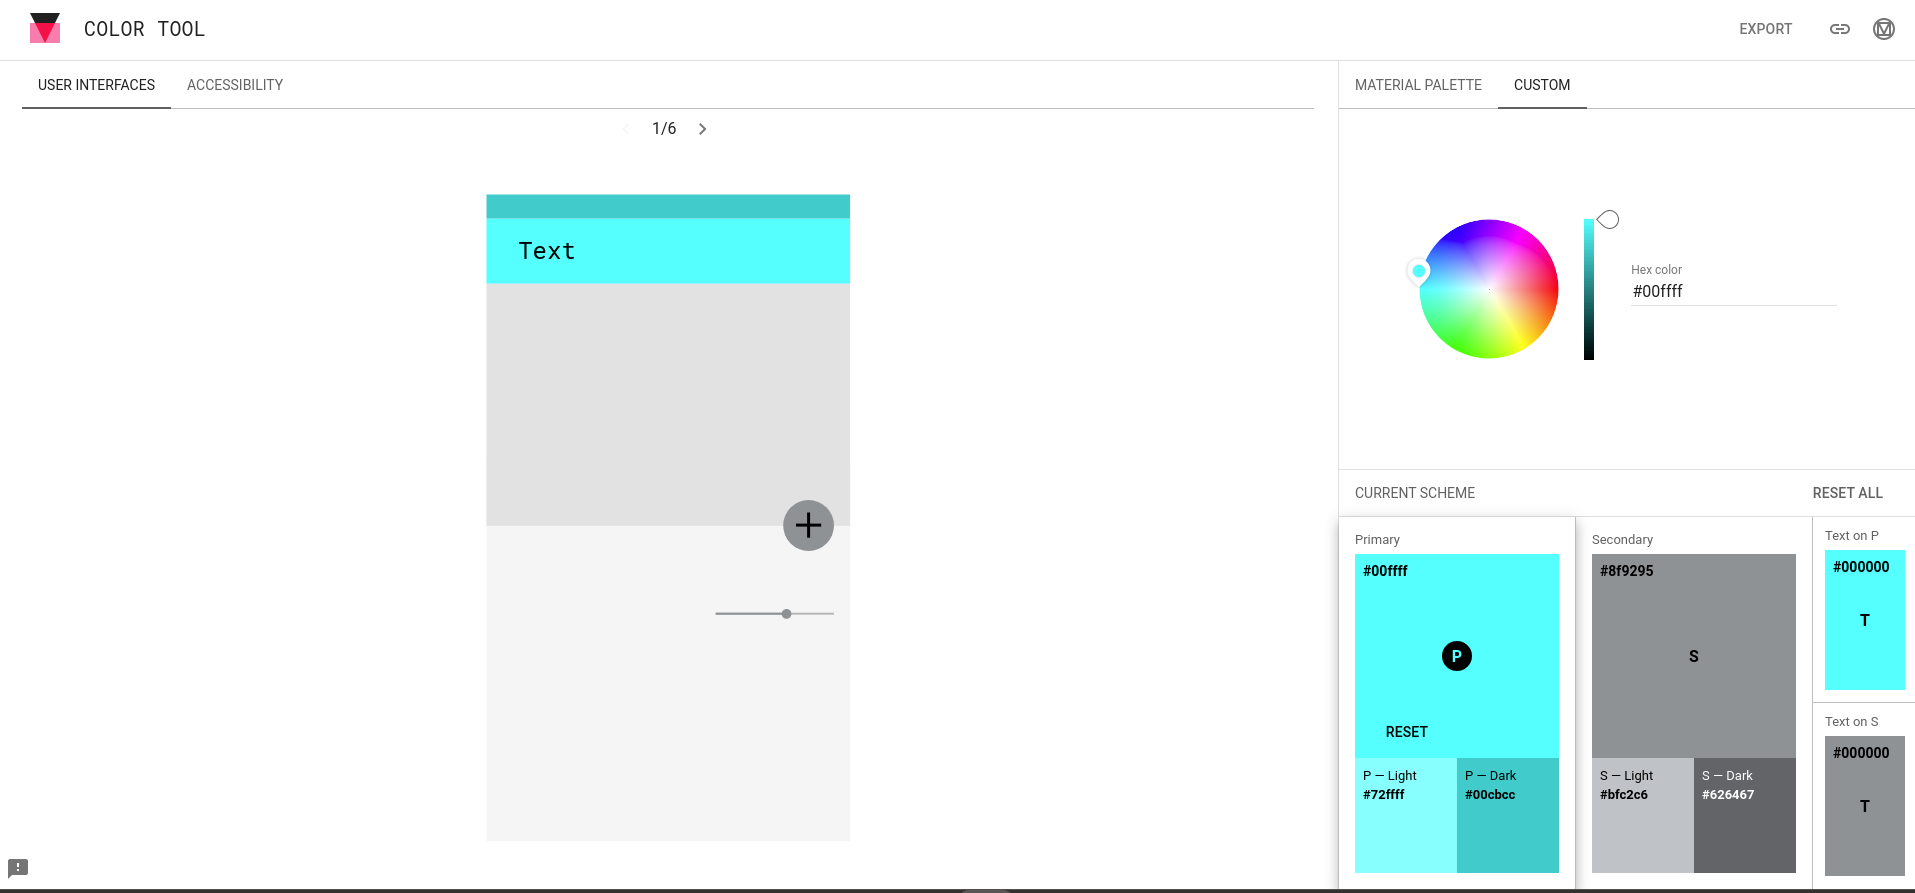
\includegraphics[width=0.5\textwidth]{capitulo1/paleta_primaria.png}
\caption{Colores primario y secundario de la aplicación}
\label{cap1:004}
\end{figure} 

Para ello editamos el archivo \textbf{lib/main.dart} quedando de la siguiente forma

\begin{lstlisting}[language=bash]
...
  @override
  Widget build(BuildContext context) {
    return MaterialApp(
      title: 'Flutter Demo',
      theme: ThemeData(
          brightness: Brightness.dark,
          primaryColor: Colors.cyan[400],
          accentColor: Colors.grey[200],
          textTheme: TextTheme(
              headline5: TextStyle(fontSize: 72.0, fontWeight: FontWeight.bold),
              headline6: TextStyle(fontSize: 36.0, fontStyle: FontStyle.italic),
              bodyText1: TextStyle(fontSize: 18.0))),
      home: MyHomePage(title: 'Flutter Demo Home Page'),
    );
  }
 ...
\end{lstlisting}

Para que el estilo de textos definidos se apliquen a los textos del app necesitamos modificarlos de la siguiente forma:

\begin{lstlisting}[language=java]
...
          children: <Widget>[
            Text(
              'You have pushed the button this many times:',
              style: Theme.of(context).textTheme.bodyText1,
            ),
            Text(
              '$_counter',
              style: Theme.of(context).textTheme.headline4,
            ),
          ],
...
\end{lstlisting}

\section{Construyendo la página de registro}
 
Para construir la página de registro, editamos primero el archivo \textbf{lib /main.dart} y le pondremos el nombre de nuestro e-commerce.

\begin{lstlisting}[language=java]
...
  @override
  Widget build(BuildContext context) {
    return MaterialApp(
      title: 'Vecnu SMARTEST e-commerce',
      theme: ThemeData(
          brightness: Brightness.dark,
          primaryColor: Colors.cyan[400],
          accentColor: Colors.grey[200],
          textTheme: TextTheme(
              headline5: TextStyle(fontSize: 72.0, fontWeight: FontWeight.bold),
              headline6: TextStyle(fontSize: 36.0, fontStyle: FontStyle.italic),
              bodyText1: TextStyle(fontSize: 18.0))),
      //home: MyHomePage(title: 'Flutter Demo Home Page'),
    );
  }
  ...
\end{lstlisting}

En el pedazo de programa de \textbf{lib /main.dart} mostrado anteriormente se realizaron dos modificaciones la primera corresponde al nombre de la aplicación la cual se llamará \textbf{Vecnu SMARTEST e-commerce} y la segunda es que la linea \textbf{home:} se convierte en comentario. La razón para hacer esto es porque vamos a borrar la clase \textbf{MyHomePage} del \textbf{lib /main.dart} y crearemos un nuevo folder en el directorio \textbf{lib} el cual llamaremos \textbf{paginas} y dentro de este directorio crearemos un programa llamado \textbf{lib /paginas /pagina\_registro.dart}

\begin{lstlisting}[language=java]
import 'package:flutter/material.dart';

class PaginaRegistro extends StatefulWidget {
  @override
  PaginaRegistroEstado createState() => PaginaRegistroEstado();
}

class PaginaRegistroEstado extends State<PaginaRegistro> {
  @override
  Widget build(BuildContext context) {
    return Text("Hola Mundo");
  }
}
\end{lstlisting}

Para poder ejecutar el programa creado activamos home: y agragamos la clase \textbf{PaginaRegistro()} anexando asimismo la libreria al programa, quedando de la siguiente manera el programa \textbf{lib /main.dart}.

\begin{lstlisting}[language=java]
import 'package:flutter/material.dart';
import 'package:vecnu/paginas/pagina_registro.dart';

void main() {
  runApp(MyApp());
}

class MyApp extends StatelessWidget {
  // This widget is the root of your application.
  @override
  Widget build(BuildContext context) {
    return MaterialApp(
      title: 'Vecnu SMARTEST e-commerce',
      theme: ThemeData(
          brightness: Brightness.dark,
          primaryColor: Colors.cyan[400],
          accentColor: Colors.grey[200],
          textTheme: TextTheme(
              headline5: TextStyle(fontSize: 72.0, fontWeight: FontWeight.bold),
              headline6: TextStyle(fontSize: 36.0, fontStyle: FontStyle.italic),
              bodyText1: TextStyle(fontSize: 18.0))),
      home: PaginaRegistro(),
    );
  }
}
\end{lstlisting}

Lo cual nos produce una salida que se muestra en la figura \ref{cap1:005}.

\begin{figure}[htb]
\centering
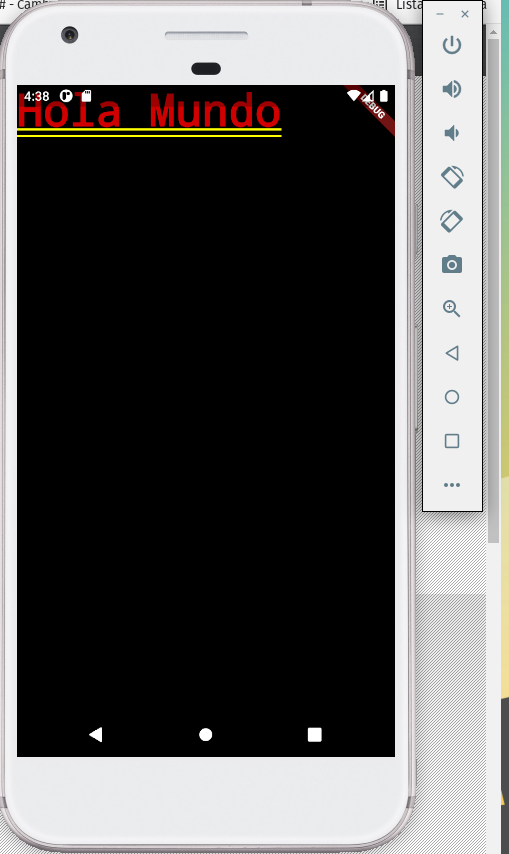
\includegraphics[width=0.3\textwidth]{capitulo1/holaMundo.png}
\caption{Salida del programa Hola Mundo}
\label{cap1:005}
\end{figure} 

\subsection{Creando el Scaffold de la página de registro}

La clase de la página de registro (\textbf{lib /paginas /pagina\_registro.dart}) la editamos y sustituimos el hola mundo por un Scaffold que tiene la estructura que deseamos. 

\begin{lstlisting}[language=java]
import 'package:flutter/material.dart';

class PaginaRegistro extends StatefulWidget {
  @override
  PaginaRegistroEstado createState() => PaginaRegistroEstado();
}

class PaginaRegistroEstado extends State<PaginaRegistro> {
  Widget _mostrarTitulo() {
    return Text(
      'Registro',
      style: Theme.of(context).textTheme.headline5,
    );
  }

  Widget _mostrarEntradaUsuario() {
    return Padding(
        padding: EdgeInsets.only(top: 20.0),
        child: TextFormField(
            decoration: InputDecoration(
                border: OutlineInputBorder(),
                labelText: 'Usuario',
                hintText: 'Introduce usuario, tamano min 6',
                icon: Icon(Icons.face, color: Colors.grey))));
  }

  Widget _mostrarEntradaCorreo() {
    return Padding(
        padding: EdgeInsets.only(top: 20.0),
        child: TextFormField(
            decoration: InputDecoration(
                border: OutlineInputBorder(),
                labelText: 'Correo',
                hintText: 'Introduce un correo valido',
                icon: Icon(Icons.mail, color: Colors.grey))));
  }

  Widget _mostrarEntradaClave() {
    return Padding(
        padding: EdgeInsets.only(top: 20.0),
        child: TextFormField(
            obscureText: true,
            decoration: InputDecoration(
                border: OutlineInputBorder(),
                labelText: 'Clave',
                hintText: 'Introduce clave, tamano min 6',
                icon: Icon(Icons.lock, color: Colors.grey))));
  }

Widget _mostrarAccionesForma() {
    final ButtonStyle raisedButtonStyle = ElevatedButton.styleFrom(
      onPrimary: Colors.black87,
      primary: Theme.of(context).primaryColor,
      minimumSize: Size(88, 36),
      padding: EdgeInsets.symmetric(horizontal: 16),
      shape: const RoundedRectangleBorder(
        borderRadius: BorderRadius.all(Radius.circular(10)),
      ),
    );
    return Padding(
      padding: EdgeInsets.only(top: 20.0),
      child: Column(
        children: [
          ElevatedButton(
            style: raisedButtonStyle,
            child: Text('Enviar',
                style: Theme.of(context)
                    .textTheme
                    .bodyText1!
                    .copyWith(color: Colors.black)),
            onPressed: () => print('Enviado'),
          ),
          TextButton(
            child: Text('Ya te registraste? Entrar'),
            onPressed: () => print('Entrar'),
          )
        ],
      ),
    );
  }


  @override
  Widget build(BuildContext context) {
    return Scaffold(
        appBar: AppBar(title: Text('Registro')),
        body: Container(
          padding: EdgeInsets.symmetric(horizontal: 20.0),
          child: Center(
            child: SingleChildScrollView(
              child: Form(
                child: Column(
                  children: [
                    _mostrarTitulo(),
                    _mostrarEntradaUsuario(),
                    _mostrarEntradaCorreo(),
                    _mostrarEntradaClave(),
                    _mostrarAccionesForma()
                  ],
                ),
              ),
            ),
          ),
        ));
  }
}

\end{lstlisting}

En programa anterior de \textbf{lib /paginas /pagina\_registro.dart} se crean 5 funciones: \_mostrarTitulo(), \_mostrarEntradaUsuario(),\_mostrarEntradaCorreo(), \_mostrarEntradaClave(), \_mostrarAccionesForma(). Todas las funciones regresan un Widget, que crea una columna de Widgets. Cada uno formando el titulo, la entrada de usuario, la entrada de correo, la clave y las formas del boton de enviar y de entrar.

\begin{figure}
\begin{subfigure}{.5\textwidth}
  \centering
  \includegraphics[width=.5\linewidth]{capitulo1/cap1:006.png}
  \caption{Pantalla de registro}
  \label{cap1:006:sfig1}
\end{subfigure}%
\begin{subfigure}{.5\textwidth}
  \centering
  \includegraphics[width=.5\linewidth]{capitulo1/cap1:006:1.png}
  \caption{click en usuario}
  \label{cap1:006:sfig2}
\end{subfigure}
\begin{subfigure}{.5\textwidth}
  \centering
  \includegraphics[width=.5\linewidth]{capitulo1/cap1:006:2.png}
  \caption{click en correo}
  \label{cap1:006:sfig3}
\end{subfigure}
\begin{subfigure}{.5\textwidth}
  \centering
  \includegraphics[width=.5\linewidth]{capitulo1/cap1:006:3.png}
  \caption{click en clave}
  \label{cap1:006:sfig4}
\end{subfigure}
\caption{Imagenes del Funcionamiento de la página de registro}
\label{cap1:006}
\end{figure}

Tambien cuando se pulsa sobre el botón \textbf{enviar} y sobre el botón \textbf{¿Ya te registraste? Entrar} se imprime en la terminal los letreros enviar y entrar 

\begin{figure}[htb]
\centering
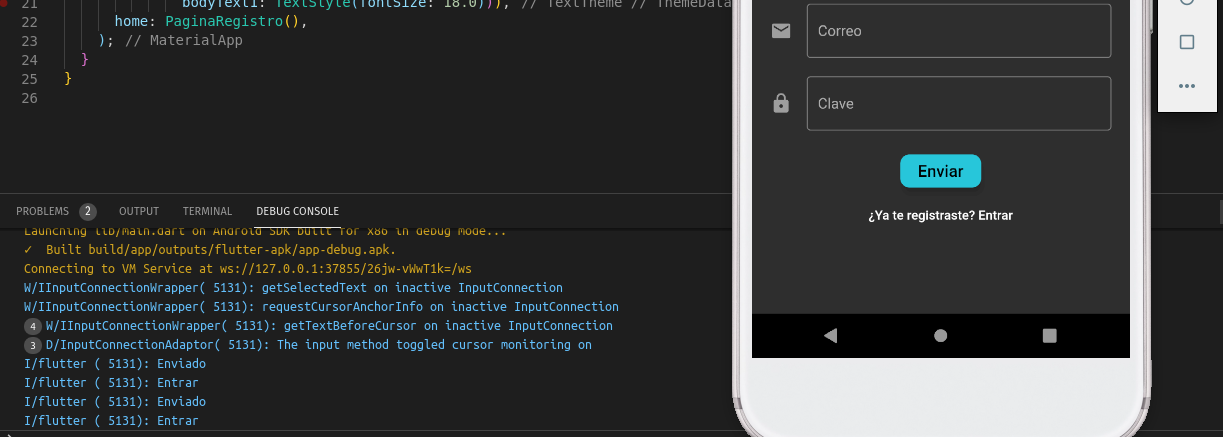
\includegraphics[width=0.5\textwidth]{capitulo1/enviar_entrar.png}
\caption{Salida al pulsar el botón \textbf{enviar} o \textbf{¿ya te registraste? enviar}}
\label{cap1:007}
\end{figure} 


\subsection{Agregando validación de forma, creando estado de forma}

Ahora agregaremos validación a la forma. Primero agregamos validación a la forma de usuario.

\begin{lstlisting}[language=java]
...
  Widget _mostrarEntradaUsuario() {
    return Padding(
        padding: EdgeInsets.only(top: 20.0),
        child: TextFormField(
            validator: (val) => val!.length < 6 ? 'Nombre usuario muy corto': null,
            decoration: InputDecoration(
...
\end{lstlisting}


Posteriormente agregamos validación a la forma de correo

\begin{lstlisting}[language=java]
...
  Widget _mostrarEntradaCorreo() {
    return Padding(
        padding: EdgeInsets.only(top: 20.0),
        child: TextFormField(
            validator: (val) => !val!.contains('@') ? 'Correo invalido':null,
            decoration: InputDecoration(
...
\end{lstlisting}

Ahora agregamos validación a la forma de clave

\begin{lstlisting}[language=java]
...
 Widget _mostrarEntradaClave() {
    return Padding(
        padding: EdgeInsets.only(top: 20.0),
        child: TextFormField(
            validator: (val) => val!.length < 6 ? 'Nombre usuario muy corto': null,
            obscureText: true,
...
\end{lstlisting}



\chapter{Diseño del servidor WEB}
Primero creamos el proyecto al cual le agregaremos la funcionalidad de excel.


\begin{lstlisting}[language=bash]
$ flutter create leer_excel
\end{lstlisting}

 Posteriormente debemos agregar el paquete de Excel a su archivo \textbf{pubspec.yaml}. Haga clic en el "excel" de arriba para obtener la última versión del paquete de Excel. Actualmente estoy usando:

\begin{lstlisting}[language=bash]
dependencies:
	excel: ^1.1.5
\end{lstlisting}

Ahora necesitamos agregar la importación de la librería, para ello creamos el archivo \textbf{\textit{leer\_excel.dart}} en donde escribiremos el programa de importación de excel.

\begin{lstlisting}[language=c]
import  'package:excel/excel.dart';
\end{lstlisting}

Se modifica el programa principal

\begin{lstlisting}[language=c]
import 'package:flutter/material.dart';
import 'package:leer_excel/leer_excel.dart';

void main() {
	runApp(const MiApp());
}

class MiApp extends StatelessWidget {
	const MiApp({Key? key}) : super(key: key);
	
	// This widget is the root of your application.
	@override
	Widget build(BuildContext context) {
		return MaterialApp(
		title: 'Lectura de Excel',
		theme: ThemeData(
		// This is the theme of your application.
		//
		// Try running your application with "flutter run". You'll see the
		// application has a blue toolbar. Then, without quitting the app, try
		// changing the primarySwatch below to Colors.green and then invoke
		// "hot reload" (press "r" in the console where you ran "flutter run",
		// or simply save your changes to "hot reload" in a Flutter IDE).
		// Notice that the counter didn't reset back to zero; the application
		// is not restarted.
		primarySwatch: Colors.blue,
		),
		home: LeerExcel(),
		);
	}
}
\end{lstlisting}

El archivo de leer\_excel.dart queda de la siguiente forma:

\begin{lstlisting}[language=java]
import 'package:excel/excel.dart';
import 'package:flutter/material.dart';
import 'dart:io';
import 'package:path/path.dart';
import 'package:excel/excel.dart';

class LeerExcel extends StatelessWidget {
	const LeerExcel({ Key? key }) : super(key: key);
	
	@override
	Widget build(BuildContext context) {
		return Container(color: const Color(0xFF2DBD3A));
	}
}
\end{lstlisting}

Cuando se intenta compilar el programa marca el siguiente error:

\begin{lstlisting}[language=java]
Error: Cannot run with sound null safety, because the following dependencies
don't support null safety
\end{lstlisting}


\subsection{Corrección en Android Studio}

Para corregir el error anterior agregamos la opción Run → Edit Configurations → Add Additional Run args → \textbf{--no-sound-null-safety}. Como se indica en la figura \ref{cap2:001}.

\begin{figure}[htb]
	\centering
	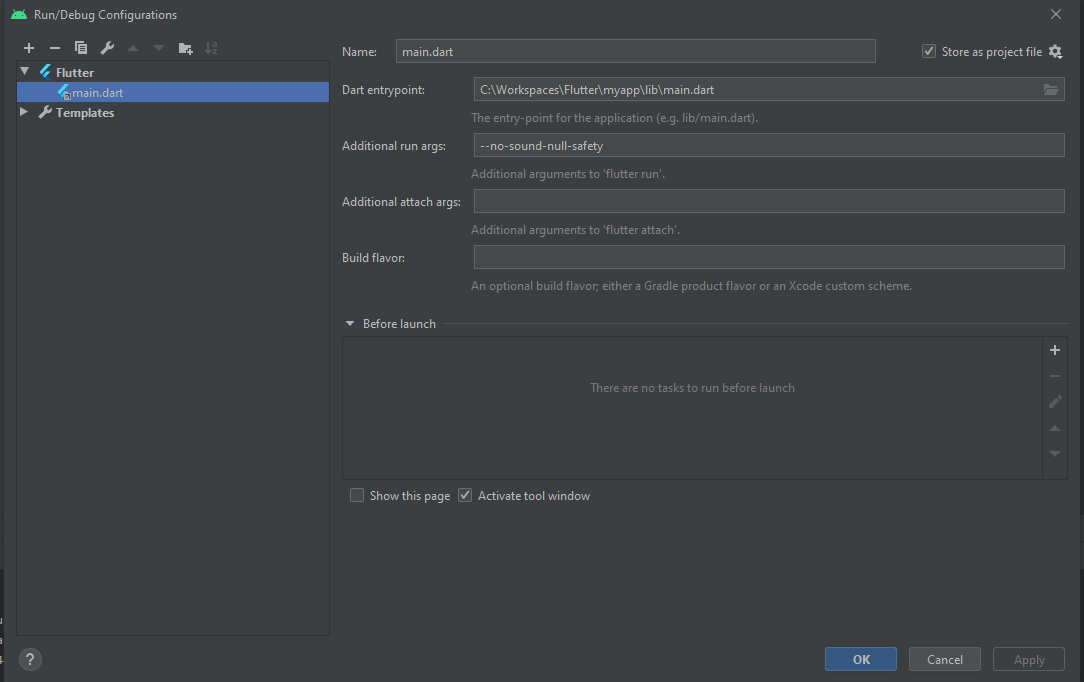
\includegraphics[width=0.7\textwidth]{capitulo2/androidstudio.png}
	\caption{Corrección del error de compilación}
	\label{cap2:001}
\end{figure} 

Después de ejecutar la compilación la salida obtenida se muestra en la figura \ref{cap2:002}.

\begin{figure}[htb]
	\centering
	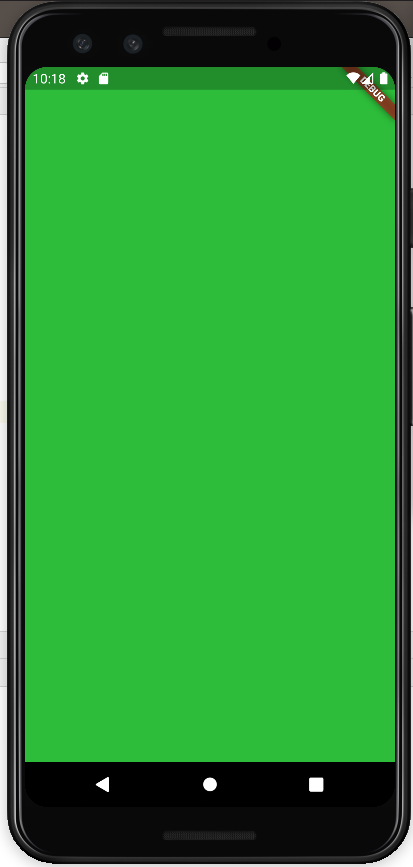
\includegraphics[width=0.4\textwidth]{capitulo2/primerPantalla.png}
	\caption{Pantalla de salida de la primera ejecución}
	\label{cap2:002}
\end{figure} 




\chapter{Procesando Solicitudes HTTP}
Primero detectamos 

\backmatter
\end{document}
